\section{Overordnede Krav}
Denne sektion skal indeholde:

\begin{itemize}
    \item Opdateret resume af overordnede krav fra inceptionsdokument
    \item Inklusiv overordnet brugsmønsterdiagram og oversigt over supplerende krav
\end{itemize}{}

% ---------------------------- Overordnede krav ------------------------------------
\subsection{Resume af Overordnede Krav}

\begin{table}[ht]
    \begin{tabularx}{\textwidth}{|p{1cm}|p{4cm}|X|}
        \hline
        \textbf{ID} & \textbf{Navn} & \textbf{Beskrivelse} \\
        \hline
        K01 & Brugergrænseflade & Systemet skal tilgås via en dansk brugergrænseflade \\
        \hline
        K02 & Brugerroller & Systemet skal indeholde brugerroller \\
        \hline
        \label{K03}K03 & Tildel roller & Kanaladministrator skal kunne tildele producer- og kanaladministrator roller \\
        \hline
        K04 & Slet bruger & Systemadministratoren skal kunne slette brugere \\
        \hline
        K05 & Se krediteringer & Alle skal kunne se krediteringer \\
        \hline
        K06 & Søg efter krediteringer & Alle skal kunne søge efter og se krediteringer for alle programmer \\
        \hline
        K07 & Opret krediteringer & Specielle brugere, kanaladministratore og systemadmin skal kunne oprette
        krediteringer for et givent program \\
        \hline
        K08 & Rediger krediteringer & Specielle brugere, kanaladmin og systemadmin skal kunne redigere krediteringer for egne programmer \\
        \hline
        K09 & Slet kreditering & Kanaladmin og systemadmin skal kunne oprette/redigere/slette krediteringer under egen kanal \\
        \hline
        K10 & Søg efter personer & Alle skal kunne søge efter personer \\
        \hline
        K11 & Knyt personer til krediteringer & Personer skal kunne knyttes til krediteringer så man kan se hvilke programmer en person har deltaget i Systemadmin, kanaladmin og producer skal kunne se persondata som email og tlf. nr. \\
        \hline
        K12 & Link personer i den virkelige verden & Det skal være muligt at linke personer i krediteringer til personer i den virkelige verden, så der krediteres korrekt \\
        \hline
        K13 & Eksporter data & Brugere skal kunne eksportere data til forskellige formater såsom XML og CSV \\
        \hline
        K14 & Importering af data & Systemet skal kunne importere EPG data via TVTid.dk \\
        \hline
        K15 & Integration & Systemet skal kunne integreres med andre systemer (Yoursee Play, Boxer Play, osv.) \\
        \hline
        K16 & Notifikationer & Systemet skal sende notifikationer til relevante brugere \\
        \hline
        K17 & Sprogvalg & Systemet skal kunne understøtte flere sprog \\
        \hline
    \end{tabularx}
    \caption{Liste af krav fra overordnet kravspecifikation} 
    \label{table:kravliste}
\end{table} 

% ---------------------------- Overordnet brugsmønsterdiagram ----------------------
\subsection{Overordnet Brugsmønsterdiagram}

\begin{figure}[H]
    \centering
    \captionsetup{justification=centering}
    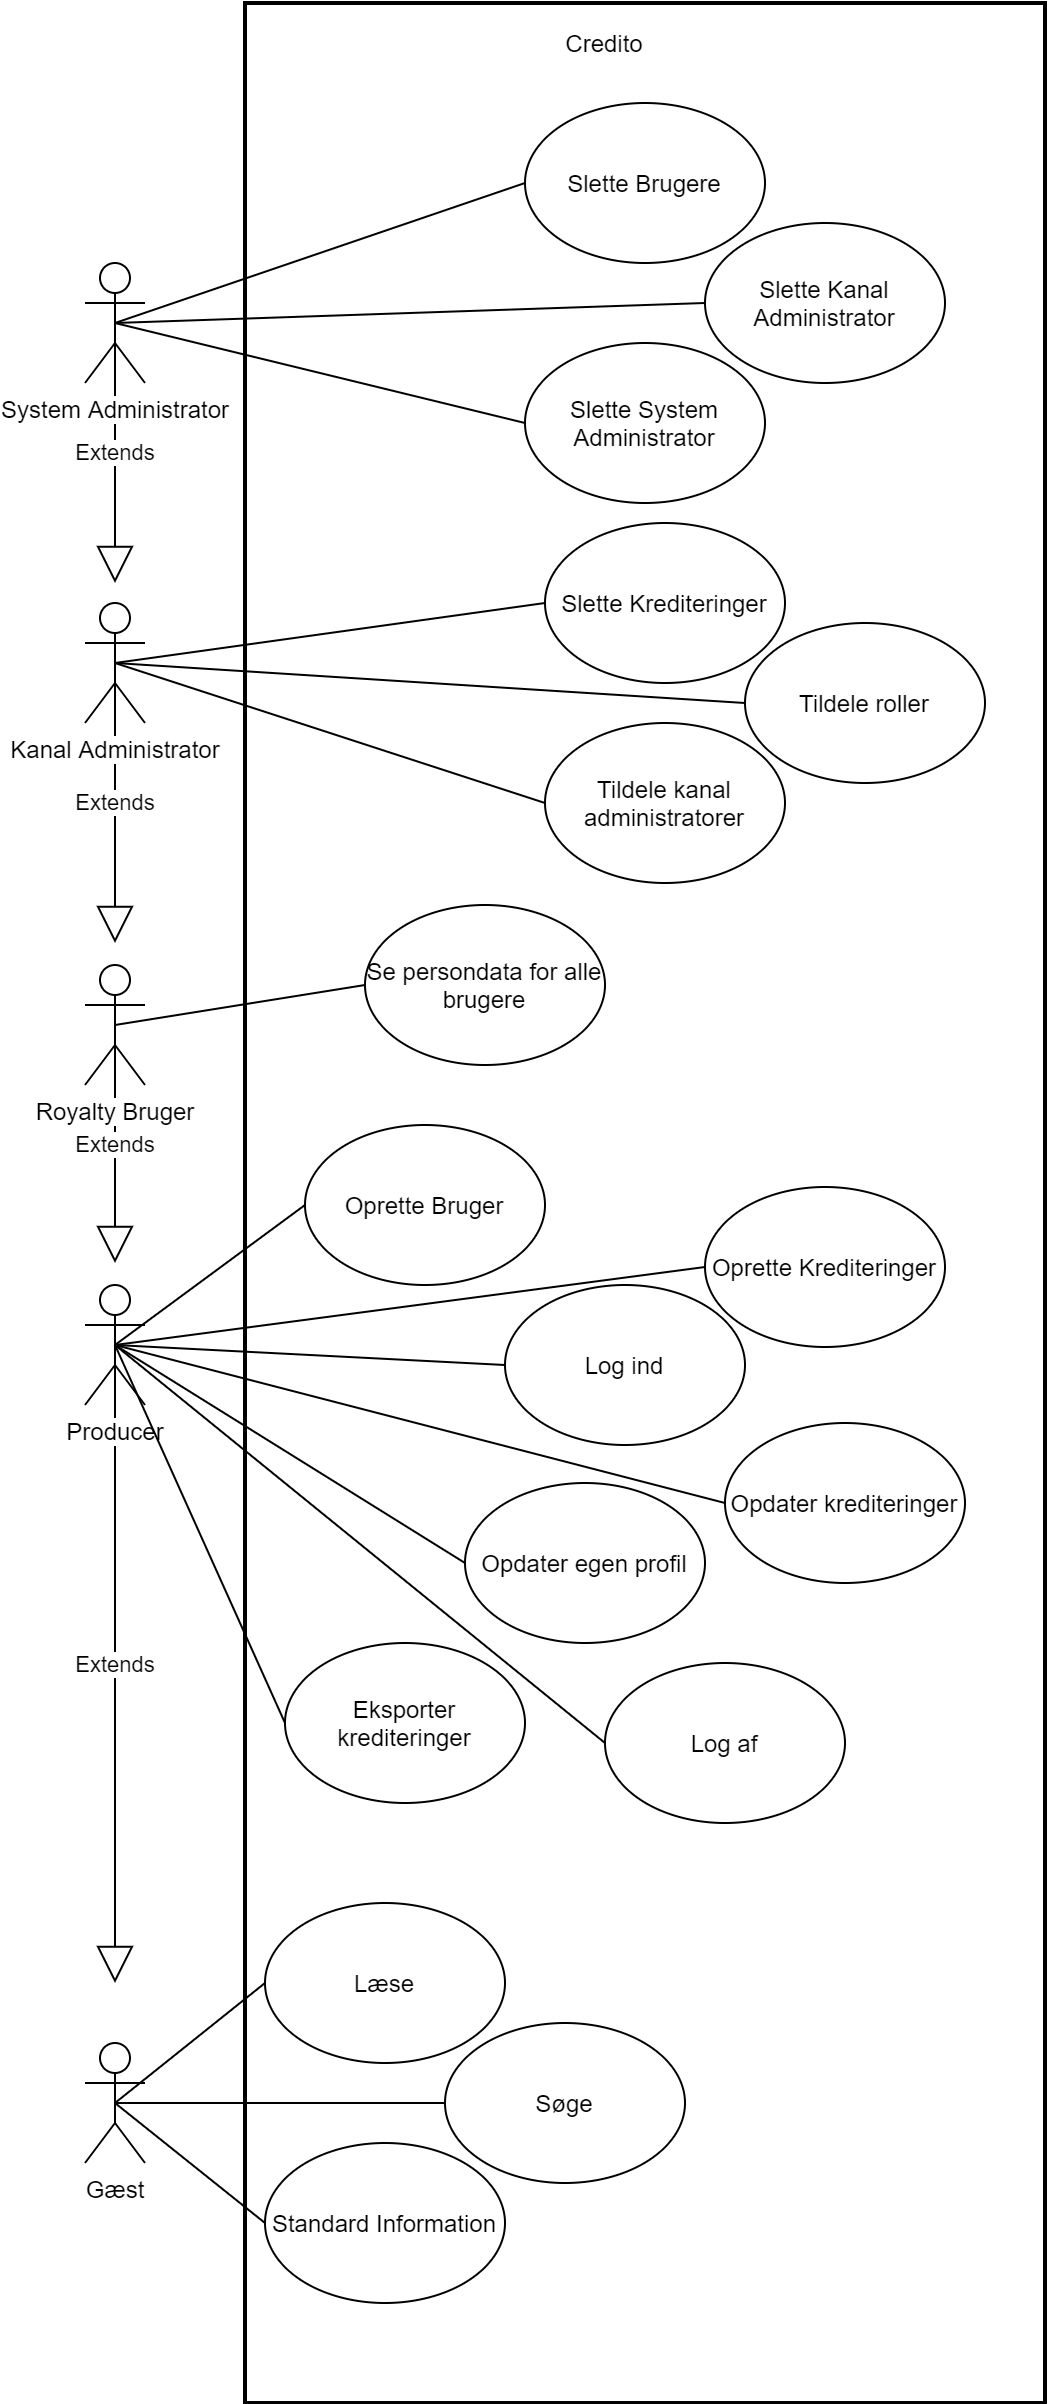
\includegraphics[scale=0.22]{figures/use-case.png}
    \caption[Overordnet brugsmønster over Creditoro systemet]%
    {Overordnet brugsmønster over Creditoro systemet 
    \par \small Menneskene er aktører. \\
    \small Cirklerne beskriver handlinger aktørne kan lave. \\
    \small Pilende betyder Extends, hvilket vil sige aktørerne arver funktionalitet}
    \label{fig:usecasemodel}
\end{figure}

% ---------------------------- Supplerende krav ------------------------------------
\subsection{Supplerende krav}

Her bruges FURPS for supplerende krav.
\begin{table}[ht]
    \begin{tabularx}{\textwidth}{|p{3cm}|X|}
        \hline
        \textbf{FURPS}           &    \textbf{Krav} \\
        \hline
        %What the customer wants! Note that this includes security-related needs.
        Functionality           & Skal kunne kreditere produktionsroller som er angivet af DRs Krediteringsregler \\
                                & Skal overholde GDPR \\
        \hline
        % How effective is the product from the standpoint of the person who must use it? Is it aesthetically acceptable? Is the documentation accurate and complete?
        Usability       & Systemet skal kunne understøtte flere sprog \\
        \hline
        % What is the maximum acceptable system downtime? Are failures predictable? Can we demonstrate the accuracy of results? How is the system recovered?
        Reliability     &  Hvis serveren til systemet genstarter, startes del-systemerne igen automatisk. Der vil ikke være behov for at ligge systemet ned regelmæssigt for at kunne foretage backup. \\
        \hline
        % How fast must it be? What's the maximum response time? What's the throughput? What's the memory consumption?
        Performance     &  Databasen skal kunne håndtere 10000 nye brugere - samt 15000 krediteringerer årligt i 25 år, uden at ofte brugte kald til REST Api'et bliver sløvt (reponsetid på mere end 300 ms) \\
        \hline
        % Is it testable, extensible, serviceable, installable, and configurable? Can it be monitored?
        Supportability  &  Systemet vil indeholde unit tests, og komme med en rapport over hvor stor en procendel der er dækket af dette. % Hvis der er mere tid kan vi indrage integrations tests?
        %Centraliseret logning (Elastic search, eller blot centraliseret system log?)
        Systemet vil blive forbundet til det centraliserede fejllognings system \texttt{Sentry}.
        Systemet er installerbart vha. Docker via Docker-compose. % (så vi blot kan sige docker-compose up -d for at få systemet op).
        Det vil være muligt at konfigurere system indstillinger via en \texttt{.env} (miljø) fil.
        En opsætningsguide vil være at finde sammen med kildekoden. 
        \\ \hline
        % The + reminds us of a few additional needs that a customer could have:
        % fx. Design constraints, Implementation requirements, interface requirements or physical requirements.
    \end{tabularx}
    \caption{FURPS}
    \label{tab:furps}
\end{table} 

\myworries{Følgende skal overvejes:}

\begin{itemize}
    \item Usability: Responsive UI
    \item Perfomance: The system should be able to handle 5000 concurrent users within a minute.
\end{itemize}
